% !TEX root = ../bachlor-arbeit.tex
\begin{tabular}{ll}
    \toprule
    Input: &
    current spectrum $I_\s c$, 
    current design parameters $\mc D$\\
    Output: & 
    improved design parameters $\mc D'$\\
    \bottomrule
\end{tabular}
\\
\\
The optimizer is at the core a Downhill-Simplex \cite{Nelder1965} tuning the continuous design parameters to minimize the mean-squared-difference between the current spectrum $I_\s{c}$ and target spectrum $I_\s{t}$ we defined as 
$C_\s{mse}\qty(I_\s{c}(p), \, I_\s{t})$.
The standard method is however unable to follow the physical constraints discussed in section \ref{sec:bg:SASA} and has to be modified in that regard. To achieve this one can introduce a distance to the boundary $D$. Let $p$ be a single continuous parameter with lower bound $p^l$ and upper bound $p^u$, then:

\begin{equation}
    D\qty(p, \, p^l, \, p^u) =
    \begin{cases}
        p^l - p, & \text{for } p < p^l\\
        0, & \text{for } p^l \leq p \leq p^u\\
        p - p^u, & \text{for } p^u < p
    \end{cases}
\end{equation}

\noindent
In this way one can penalize the simplex for stepping over the set boundaries by using a total loss $L$ which depends on the sum of all distances $D_i$:

\begin{equation}
    L(I_\s{c}, \,I_\s{t}, \,p) =
    {\underbrace{%
    \vphantom{ \left(\frac{a^{0.3}}{b}\right) }
    C_\s{mse}(I_\s{c}, \, I_\s{t})}_{\text{find target}}}
    +
    {\underbrace{%
    \qty[\sum_i D\qty(p_i, \, p_i^l, \, p_i^u)]^2
    }_{\text{stay within bounds}}}\\
\end{equation}

The choice of power depends on how much the simplex should be penalized for stepping over a boundary. All our conditions are requirements for physical approximations and these approximations do no break completely when a boundary is only slightly violated. That justifies this approach where the simplex might step over a boundary but is then "pushed back" in the right direction. 

\begin{figure}[H]
    \floatbox[{\capbeside\thisfloatsetup{capbesideposition={right,top},capbesidewidth=6.5cm}}]{figure}[\FBwidth]
    {\caption*{
    Step 0: \\
    This is the userinterface of the algorithm. In blue we can see the target spectrum $I_\s t$ which is in this case a random stack of the validation data and the current spectrum $I_\s c$ is shown in orange. In the right window all the current stack parameters are shown and at the very bottom we can see the current loss. This is the situation right after the network has made its prediction and the optimizer has not changed any parameters.}
    \label{fig:al:same_spec}}
    {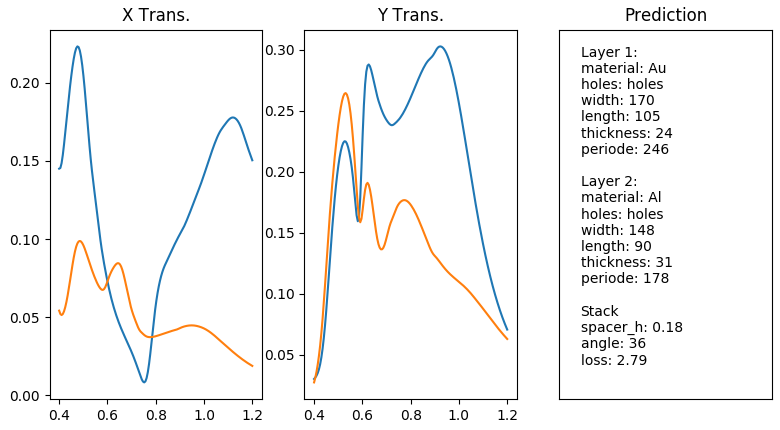
\includegraphics[width=.6\textwidth]{al_step_0}}
\end{figure}

\begin{figure}[H]
    \floatbox[{\capbeside\thisfloatsetup{capbesideposition={right,top},capbesidewidth=6cm}}]{figure}[\FBwidth]
    {\caption*{
    Step 50: \\
    After 50 steps we can see the optimizer has tuned the continuous parameters and left the material and geometry unchanged. The loss has halved and the target and current spectrum look visually more similar.}
    \label{fig:al:same_spec}}
    {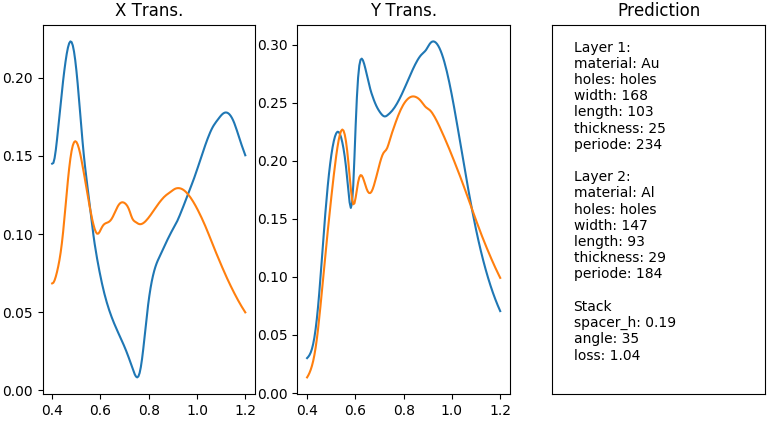
\includegraphics[width=.6\textwidth]{al_step_50}}
\end{figure}

\begin{figure}[H]
    \floatbox[{\capbeside\thisfloatsetup{capbesideposition={right,top},capbesidewidth=6cm}}]{figure}[\FBwidth]
    {\caption*{
    Step 150:\\
    As the target spectrum is in this cased produced by a know stack the optimizer should be able to reproduce it perfectly.
    }
    \label{fig:al:same_spec}}
    {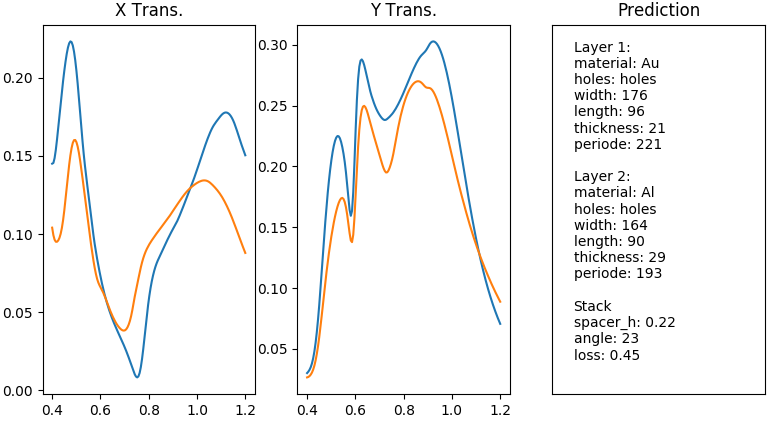
\includegraphics[width=.6\textwidth]{al_step_150}}
\end{figure}

\begin{figure}[H]
    \floatbox[{\capbeside\thisfloatsetup{capbesideposition={right,top},capbesidewidth=6cm}}]{figure}[\FBwidth]
    {\caption*{
    Step 250:\\
    This is the final result. The optimizer has gotten close to the target but there are still some slight differences. We can compare the result to the true parameters used for the generation of this spectrum seen in the figure below.
    }
    \label{fig:al:same_spec}}
    {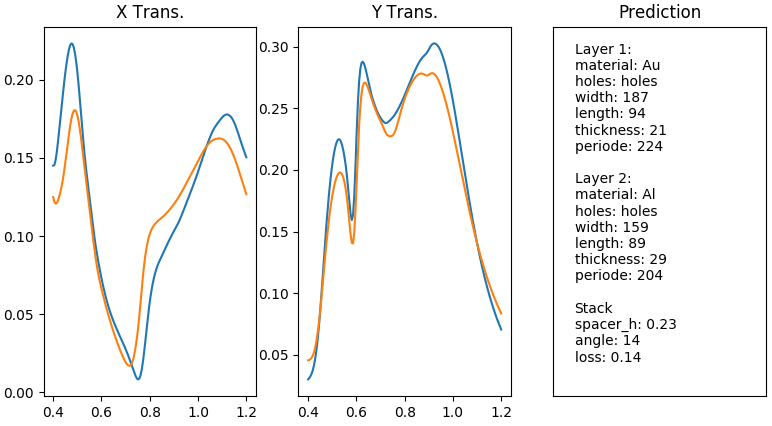
\includegraphics[width=.6\textwidth]{al_step_250}}
\end{figure}

\begin{figure}[H]
    \floatbox[{\capbeside\thisfloatsetup{capbesideposition={right,top},capbesidewidth=6cm}}]{figure}[\FBwidth]
    {\caption*{
    }
    \label{fig:al:same_spec}}
    {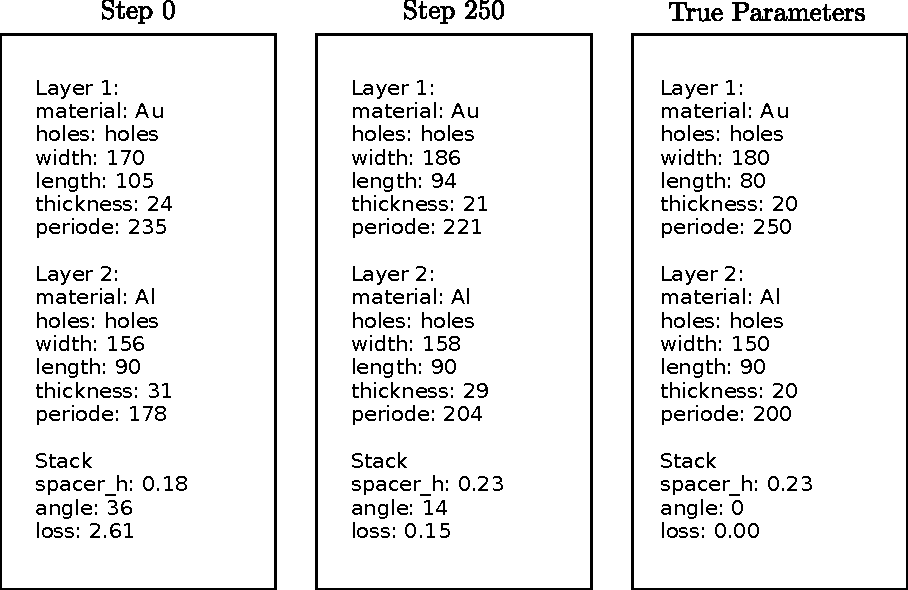
\includegraphics[width=.6\textwidth]{al_true_params}}
\end{figure}